\chapter{Les lentilles}

\section{Propagation dans les diélectriques}
\begin{wrapfigure}[10]{l}{5.5cm}
	\vspace{-5mm}
	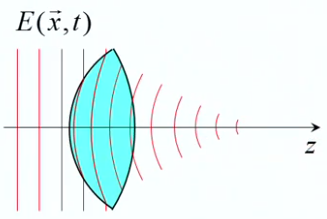
\includegraphics[scale=0.45]{ch3/image1.png}
	\captionof{figure}{ }
	\end{wrapfigure}	
Les lentilles étant faites en matériau diélectriques, il est intéressant de s'y attarder. Un diélectrique 
est un milieu constitués d'atomes qui conservent leurs électrons (à la différence des conducteurs). Si on 
place un atome dans un champ électrique, les deux vont se de façon opposés (étant de charge opposée) sur 
un distance $x(t)$ (le champ électrique dépendant du temps). Ceci donne lieu à un dipôle oscillant.\\

\begin{wrapfigure}[6]{r}{9cm}
	\vspace{-5mm}
	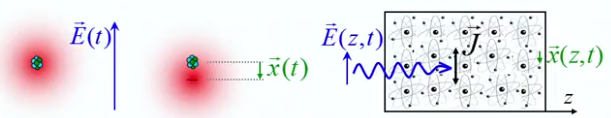
\includegraphics[scale=0.45]{ch3/image2.png}
	\captionof{figure}{ }
	\end{wrapfigure}
Dans un matériau diélectrique, on aura une vibration $\vec{x}(z,t)$ où $z$ est la coordonnée de propagation. 
Ceci donne lieur à des mouvements de charges dépendant de la position et du temps. Comme ces charges bougent, 
elles créent une densité de courant. On définit ainsi la \textit{densité de courant des charges liées}
\begin{equation}
\vec{J} = \eta_aq\dfrac{\partial \vec{x}}{\partial t}
\end{equation}
L'idée est d'aborder ça avec les équations de Maxwell
\begin{equation}
\left\{\begin{array}{ll}
\rot \vec{E} &= -\dfrac{\partial \vec{B}}{\partial t}\\
\rot \vec{B} &= \mu_0\vec{J} + \mu_0\epsilon_0\dfrac{\partial \vec{E}}{\partial t}
\end{array}\right.
\end{equation}
En prenant le rotationnel de la première équation
\begin{equation}
\rot(\rot\vec{E}) = -\dfrac{\partial \rot\vec{B}}{\partial t} = -\mu_0\dfrac{\partial \vec{J}}{\partial 
t} - \mu_0\epsilon_0\dfrac{\partial^2\vec{E}}{\partial t^2}
\end{equation}
La divergence étant nulle, le rotationnel du rotationnel donne $-\Delta$ ce qui donne, après simplification 
des signes négatifs
\begin{equation}
\Delta \vec{E} = \mu_0\dfrac{\partial\vec{J}}{\partial t}+\mu_0\epsilon_0\dfrac{\partial^2\vec{E}}{\partial 
t^2}
\end{equation}
En considérant le cas à une dimension en en faisant passer le second terme dans le membre de gauche :
\begin{equation}
\dfrac{\partial^2\vec{E}}{\partial z^2} - \dfrac{1}{c^2}\dfrac{\partial^2\vec{E}}{\partial t^2} = \mu_0 
\dfrac{\partial\vec{J}}{\partial t}
\end{equation}
On retrouve exactement l'équation d'onde sans le terme de densité de courant de charges liées : le milieu 
introduit un terme en $\vec{J}$ un peu comme un terme de source. Avec l'expression de $\vec{J}$ :
\begin{equation}
\dfrac{\partial^2\vec{E}}{\partial z^2} - \dfrac{1}{c^2}\dfrac{\partial^2\vec{E}}{\partial t^2} = \mu_0 \eta_a 
q \dfrac{\partial^2\vec{x}}{\partial t^2}
\end{equation}

\begin{wrapfigure}[8]{l}{4cm}
	\vspace{-2mm}
	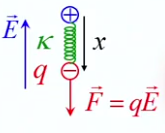
\includegraphics[scale=0.55]{ch3/image3.png}
	\captionof{figure}{ }
	\end{wrapfigure}
On voit apparaître l'accélération des charges et non pas un mouvement de translation qui génère des ondes. 
Notons que $\vec{x}$ est bien fonction du champ : comment $\vec{x}$ évolue en fonction du champ. Ceci 
permettra de "fermer" l'équation et ainsi de la résoudre. Pour se faire, adoptons le modèle des ressorts 
de Lorentz : le nuage électronique est lié aux noyaux comme une masse fixée à un ressort. Il est dès lors 
possible de lier ces deux variables. En faisant ceci, on réalise que l'on peut obtenir la solution suivante\footnote{
Les détails ne sont pas repris ici, c'est du rappel (cf. BA1).}
\begin{equation}
E(z,t) = E_\omega \cos[k(\omega)z-\omega t]
\end{equation}
La seule différence par rapport à la propagation dans le vide est que l'expression $k(\omega)$ est non 
triviale (dans le vide $k=\omega/c$). La résolution de l'équation d'onde (dérivée double par rapport à 
$z$) donne lieu à
\begin{equation}
k^2=\dfrac{\omega^2}{c^2}+\omega^2\mu_0\epsilon_0\chi(\omega) = \dfrac{\omega^2}{c^2}[1+\chi(\omega)]
\end{equation}
où $\chi(\omega)$ est la susceptibilité du milieu. Cette simple fonction contient l'information relative 
au movement des charges dans le diélectrique. En utilisant la \textit{perméabilité relative du mileu} 
$\epsilon_r = [1+\chi(\omega)]$, on peut écrire
\begin{equation}
k(\omega) = \dfrac{\omega}{c}\sqrt{\epsilon_r(\omega)} = \dfrac{\omega}{c} n(\omega)
\end{equation}
où $n(\omega) \equiv \sqrt{\epsilon_r(\omega)}$ est l'indice de réfraction. Il s'agit d'une fonction 
qui contient toute la dynamique des charges mises en mouvement par le champ électrique lui même, elle 
reforme toute la complexité microscopique. On peut montrer que $c/n(\omega)$ est la \textit{vitesse de 
propagation (phase) de la lumière dans un diélectrique}\footnote{Pour le voir, mettre $k(\omega)$ en évidence 
dans la solution de l'équation d'onde $E(z,t)$.}
\begin{equation}
\hookrightarrow k(\omega) = \dfrac{\omega}{c}\sqrt{\epsilon_r(\omega)} = \dfrac{\omega}{c} n(\omega) = 
\dfrac{\omega}{v}
\end{equation}
L'indice de réfraction est le facteur de diminution de la vitesse de l'onde dans un diélectrique, 
l'indice de réfraction étant toujours plus grande que l'unité.
\begin{equation}
v = \frac{c}{n}
\end{equation}


Tout se base la dessus. Étudions une lame de matériau diélectrique (verre) traversée par une onde 
plane monochromatique :
\begin{equation}
E(z,t) = E_\omega \cos[kz-\omega t]
\end{equation}
\newpage
\begin{wrapfigure}[8]{l}{6.4cm}
%	\vspace{-2mm}
	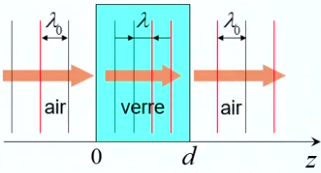
\includegraphics[scale=0.55]{ch3/image4.png}
	\captionof{figure}{ }
	\end{wrapfigure}
Avant de rentrer dans la lentille, l'onde plane se propage dans le vide : $k= k_0$ soit le 
nombre d'onde dans le vide et $\lambda_0 = \frac{2\pi}{k_0}$ la longueur d'onde dans le vide. Dans 
le milieu diélectrique, il ne faut \textbf{pas} reprendre $k_0$ mais $k = k_0n$ : la longueur 
d'onde sera plus petite, divisée par $n$, l'indice de réflexion est également le facteur de diminution 
de la longueur d'onde : $\lambda = \lambda_0/n$. \\

Interprétons ceci en nous basant sur la vitesse dans le diélectrique 
\begin{equation}
v = \frac{\omega}{n} = \frac{\omega}{k_0n} = \frac{c}{n}
\end{equation}

\begin{wrapfigure}[8]{r}{6.4cm}
	\vspace{-10mm}
	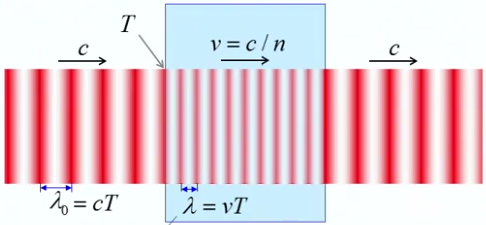
\includegraphics[scale=0.35]{ch3/image5.png}
	\captionof{figure}{Dans le vide $\lambda_0=cT$ et dans le verre $\lambda = vT$.}
	\end{wrapfigure}
La vitesse dans le diélectrique est moindre (les fronts d'ondes paraissent plus rapprochés), mais la 
période reste bien sûr inchangée. Le 
diélectrique cause un \textit{déphasage} : dans le diélectrique un front d'onde va "moins loin" que 
s'il était dans le vide (les fronts d'ondes seraient plus espacés), il y a donc distorsion de phase.\\


\begin{wrapfigure}[6]{l}{4.4cm}
	\vspace{-5mm}
	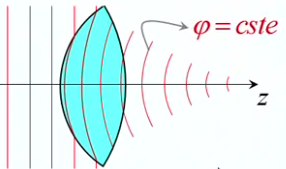
\includegraphics[scale=0.35]{ch3/image6.png}
	\captionof{figure}{ }
	\end{wrapfigure}
Une lentille c'est une lame à épaisseur variable causant un retard de phase variable (plus l'épaisseur 
de verre traversée est grande, plus cet effet de déphasage sera important). Les lieux de points de phases 
constantes, les fronts d'ondes, seront des surfaces à priori courbes.\\

Comme nous nous intéressons à la phase, aux fronts d'onde, regardons le phaseur
\begin{equation}
E(z,t) = E_\omega e^{ikz}e^{-i\omega t}
\end{equation}
La phase accumulée sur l'épaisseur $d$ sera forcément $\varphi = kd = nk_0d$. Sans la lame de verre 
$\varphi = k_0d$. Le \textit{retard de phase (déphasage)} est obtenu en comparant la phase accumulée 
dans le verre avec celle dans le vide pour la même longueur traversée c'est à dire $d$
\begin{equation}
\Delta\varphi = k_0d(n-1)
\end{equation}
\textbf{Remarque} : Un retard de phase est une phase qui évolue plus vite dans le diélectrique, mais 
il faut se souvenir que pour une distance donnée on a une "plus grande densité de fronts d'onde". Phase 
qui évolue rapidement veut dire retard de phase.\\
































